\documentclass[dvipdfmx, tikz]{standalone}
\usepackage{tikz}
\usetikzlibrary{calc,decorations.pathreplacing,quotes,positioning,shapes,fit,arrows,backgrounds,tikzmark}

\begin{document}
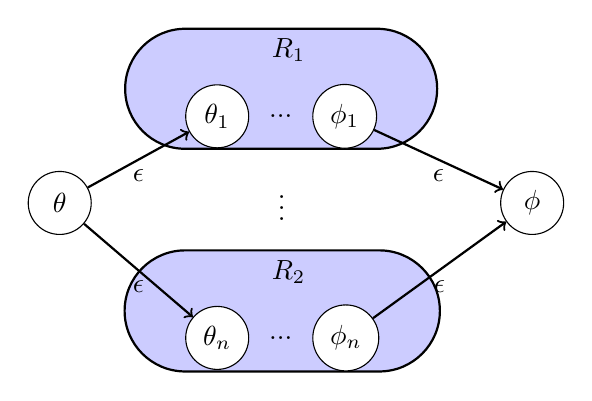
\begin{tikzpicture}[state/.style={circle, draw, fill=white, minimum size=.8cm}, node distance=.8cm]
	\node(a0) [state] at (0,0) {$\theta_1$};
	\node(a1) [state, right =of a0] {$\phi_1$};
	\node(a2) [state, below =2cm of a0] {$\theta_n$};
	\node(a3) [state, right =of a2] {$\phi_n$};
	
	\node(n1) [above right=.4cm of a0, minimum size=0] {$R_1$};
	\node(n2) [above right=.4cm of a2, minimum size=0] {$R_2$};
  \node(s) [state] at (-2, -1.1) {$\theta$};
  \node(g) [state] at (4, -1.1) {$\phi$};

  \draw[->, thick] (s) -- node(e0)[midway, below] {$\epsilon$} (a0);
  \draw[->, thick] (s) -- node(e1)[midway, below] {$\epsilon$} (a2);
  \draw[->, thick] (a1) -- node(e2)[midway, below] {$\epsilon$} (g);
  \draw[->, thick] (a3) -- node(e3)[midway, below] {$\epsilon$} (g);

	\draw[draw opacity=0] (a0) -- node[midway] {...} (a1);
	\draw[draw opacity=0] (a2) -- node[midway] {...} (a3);
	\begin{scope}[on background layer]
	\node(R1)[fill=blue!20, draw=black, thick,rounded rectangle, inner sep=0cm, fit=(a0) (a1) (n1)] {};
	\node(R2)[fill=blue!20, draw=black, thick,inner sep=0cm, rounded rectangle, fit=(a2) (a3) (n2)] {};
	\draw[draw opacity=0] (R1) -- node[midway] {$\vdots$} (R2);
	\end{scope}
  \ifx\TNFAActivateEdgeLabel\undefined \else
    \node[above left=0 of e0] {$s\mathchar`-edge$};
    \node[left=0 of e1] {$s\mathchar`-edge$};
    \node[above right=0 of e2] {$g\mathchar`-edge$};
    \node[right=0 of e3] {$g\mathchar`-edge$};
  \fi
	
\end{tikzpicture}
\end{document}
